\section{Infinitesimal Lorentz Transformations}

In this section the infinitesimal Lorentz transformations are derived. These transformations can be used to determine the equations of motion of a particle as it travels through Minkowskian space-time. It is interesting to write these equations in terms of the particles $3$-velocity as the form of the Lorentz force emerges. It is shown that the Lorentz force must depend on the particle's $3$-velocity in a special way in order to be compatible with special relativty. Then the fractional linear transformation associated with the infinitesimal transformation is derived to find that the resulting radiation field must be a pure radiation field. Finally the conditions for a pure radiation field are extended to Minkowskian space-time.

The Infinitesimal transformations are Lorentz transformations that are small perturbations of the identity transformation and so $U \in SL(2,\mathbb{C})$ has the form

\begin{equation}\label{Infinitesimal_Infinitesimal_Lorentz_Transform_Matrix_U}
U = \pm
\left(
\begin{array}{cc}
1 + \epsilon a & \epsilon b \\
\epsilon c & 1 + \epsilon f \\
\end{array}
\right),
\end{equation}

\noindent where $a,b,c,f \in \mathbb{C}$ and $\epsilon$ is a small real parameter. Here terms of order $\epsilon^2$ will be neglected. As $U \in SL(2,\mathbb{C})$ its determinant is calculated as

\begin{equation*}
\det{(U)} = 1 + O(\epsilon^2).
\end{equation*}

\noindent Using this it is possible to obtain a relation between $f$ and $a$

\begin{gather*}
(1 + \epsilon a)(1 + \epsilon f) - \epsilon^2 b c = 1 + O(\epsilon^2), \\
1 + \epsilon (a +f) = 1 + O(\epsilon^2), \\
f = -a + O(\epsilon).
\end{gather*}

\noindent Hence 

\begin{equation}\label{Infinitesimal_Infinitesimal_Lorentz_Transform_Matrix_U_Final}
U =
\left(
\begin{array}{cc}
1 + \epsilon a & \epsilon b \\
\epsilon c & 1 - \epsilon a \\
\end{array}
\right).
\end{equation}

Now the explicit infinitesimal Lorentz transformations are calculated as in section \ref{Special_Linear_Matrices_of_Lorentz}, by substituting $U$ into

\begin{equation*}
A(\vec{x}') = U A(\vec{x}) U^{\dagger}.
\end{equation*}

\noindent Writing this out in component form gives

\begin{align*}
\left(
\begin{array}{cc}
t'-z' & x' + iy' \\
x' - iy' & t'+z' \\
\end{array}
\right)
=
\left(
\begin{array}{cc}
1 + \epsilon a & \epsilon b \\
\epsilon c & 1 - \epsilon a \\
\end{array}
\right)
\left(
\begin{array}{cc}
t-z & x + iy \\
x - iy & t+z \\
\end{array}
\right)
\left(
\begin{array}{cc}
1 + \epsilon  \bar{a} & \epsilon \bar{c} \\
\epsilon \bar{b} & 1 - \epsilon \bar{a} \\
\end{array}
\right), \\
=
\left(
\begin{array}{cc}
1 + \epsilon a & \epsilon b \\
\epsilon c & 1 - \epsilon a \\
\end{array}
\right)
\left(
\begin{array}{cc}
(t-z)(1 + \epsilon \bar{a})+\epsilon \bar{b}(x + iy) & (t-z)\epsilon \bar{c}+ (1 - \epsilon \bar{a})(x + iy) \\
(x - iy)(1 + \epsilon \bar{a}) +\epsilon \bar{b} (t+z) & (x - iy)\epsilon \bar{c}+(1 - \epsilon \bar{a})(t+z) \\
\end{array}
\right).
\end{align*}

\noindent This then implies the three relations

\begin{eqnarray}\label{Infinitesimal_Lorentz_Transform_1}
t'-z' = t-z + \epsilon(a + \bar{a})(t-z) + \epsilon(b + \bar{b})x + i\epsilon(\bar{b} - b)y + O(\epsilon^2), \\\label{Infinitesimal_Lorentz_Transform_2}
t'+z' = t+ z - \epsilon(a + \bar{a})(t+z) + \epsilon (c + \bar{c})x + i \epsilon(c-\bar{c})y + O(\epsilon^2), \\\label{Infinitesimal_Lorentz_Transform_3}
x'+iy' = x+iy + \epsilon(a-\bar{a})(x+iy) + \epsilon(b + \bar{c})t + \epsilon (b-\bar{c})z + O(\epsilon^2).
\end{eqnarray}

\noindent As $a,b,c \in \mathbb{C}$, set 

\begin{equation*}
a = a_1 +ia_2 \text{,  } b = b_1 +ib_2 \text{,  } c = c_1 +ic_2 \text{.} 
\end{equation*}

\noindent Then subbing these into the above equations, eliminating $t$ and $z$ respectively from Eqn.(\ref{Infinitesimal_Lorentz_Transform_1}) and (\ref{Infinitesimal_Lorentz_Transform_2}) and taking real and imaginary parts of Eqn.(\ref{Infinitesimal_Lorentz_Transform_3}) to obtain

\begin{equation}\label{infinitesimal_Matrix_component_wise}
\left(
\begin{array}{c}
x' \\
y'\\
z'\\
t'\\
\end{array}
\right)
=
\left(
\begin{array}{c}
x \\
y\\
z\\
t\\
\end{array}
\right)
+ \epsilon
\left(
\begin{array}{cccc}
0            & -2a_2        & (b_1 - c_1) & (b_1+c_1)\\
2a_2         & 0            & (b_2+c_2)   & (b_2 - c_2) \\
-(b_1 - c_1) & -(b_2 + c_2) & 0           & -2a_1 \\
(b_1 + c_1)  & (b_2-c_2)    & -2a_1       & 0 \\
\end{array}
\right)
\left(
\begin{array}{c}
x \\
y\\
z\\
t\\
\end{array}
\right)
+ O(\epsilon^2).
\end{equation}

\noindent The above $4 \times 4$ matrix will be denoted as $\tensor{L}{^i_j}$, so that Eqn.(\ref{infinitesimal_Matrix_component_wise}) can be written simply as 

\begin{equation}\label{Infinitesimal_Infinitesimal_Lorentz_Transformation}
\bar{x}^i = x^i + \epsilon \tensor{L}{^{i}_{j}} x^j + O(\epsilon^2),
\end{equation}

\noindent where $\bar{x}^i = (x',y',z',t')$. It is also necessary to check that the Lorentz invariance of the quadratic form still holds. 

\begin{align*}
{x'}^2 + {y'}^2 + {z'}^2 - {t'}^2 & = x^2 + y^2 + z^2 - t^2 - 4\epsilon a_2 x y + 2 \epsilon(b_1 + c_1)xt \\
                                  & + 2\epsilon (b_1 - c_1)xz + 4 \epsilon a_2 yx + 2\epsilon (b_2 - c_2)yt \\
                                  & + 2 \epsilon (b_2 + c_2)yz - 4\epsilon a_1 zt + 2 \epsilon (c_1 - b_1)zx \\
                                  & -2 \epsilon (c_2 + b_2)zy + 4 \epsilon a_1 tz - 2 \epsilon (c_1 + b_1)tx \\
                                  & -2\epsilon (b_2 - c_2) ty + O(\epsilon^2) \\
                                  & = x^2 + y^2 + z^2 - t^2 + O(\epsilon^2)
\end{align*}

\noindent Hence this transformation is still a Lorentz Transformation if we neglect terms of order $\epsilon^2$.

Consider the time-like world line of a particle in Minkowskian space-time $x^i = x^i(s)$. If $s$ is arc length or proper time then $v^i(s) = \frac{dx^i}{ds}$ is the unit tangent vector field. It is clear that $v^i(s)$ must be time-like as $x^i(s)$ is time-like, thus

\begin{equation*}
\eta_{ij} v^i v^j = -1,
\end{equation*}

\noindent where $\eta_{ij} = \text{diag}(1,1,1,-1)$ is the metric of Minkowskian space-time. This implies that 

\begin{equation*}
(v^1)^2  + (v^2)^2 + (v^3)^2  - (v^4)^2 = -1.
\end{equation*}

Now consider taking a step along the world line of the particle. Define $\bar{s} = s + \alpha$, where $\alpha$ is some real parameter, so that $v^i (s+\alpha) \vcentcolon = \bar{v}^i(\bar{s})$, see Fig.(\ref{Infinitesimal_Fig_Steps_Along_Minkowskian}).

\begin{figure}[h!]
\begin{center}
\caption{\textit{The trajectory of a particle moving through Minkowskian space time. The position along the path is parameterised by $s$. A step along the curve from $s$ to $s+\alpha$ is shown. This step is found to be a Lorentz transformation as both $v^i(s)$ and $\bar{v}^i(\bar{s})$ have equal Lorentz quadratic forms.}}
\label{Infinitesimal_Fig_Steps_Along_Minkowskian}
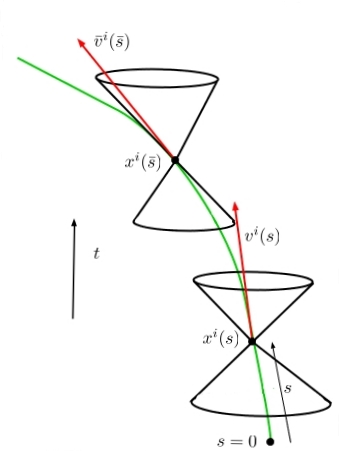
\includegraphics[scale=0.8]{figs/5_4.jpg}
\end{center}
\end{figure}

Hence we also have

\begin{equation*}
({\bar{v}^1})^2  + ({\bar{v}^2})^2 + ({\bar{v}^3})^2  - ({\bar{v}^4})^2 = -1,
\end{equation*}

\noindent and so $v^i(s)$ and $\bar{v}^i(\bar{s})$ are related by a Lorentz transformation. In particular $v^i(s+\epsilon)$ and $v^i(s)$ are related by an infinitesimal Lorentz Transformation given by Eqn.(\ref{Infinitesimal_Infinitesimal_Lorentz_Transformation}),

\begin{equation}
v^i(s+\epsilon) = v^i(s) + \epsilon \tensor{L}{^{i}_{j}}(s)v^j (s) + O(\epsilon^2).
\end{equation}

\noindent Rearranging to obtain

\begin{equation}
\frac{v^i(s+\epsilon) - v^i(s)}{\epsilon} = \tensor{L}{^{i}_{j}}(s)v^j (s) + O(\epsilon).
\end{equation}

\noindent Now taking the limit as the infinitesimal step, $\epsilon$ goes to zero to obtain a continuous differential equation,

\begin{equation}\label{Infinitesimal_DE_interms_v}
\frac{dv^i}{ds} = \tensor{L}{^{i}_{j}}(s) v^j (s).
\end{equation}

\noindent This equation determines the trajectory of the particle through Minkowskian space-time. In terms of $x$ this is equivalent to

\begin{equation*}
\frac{d^2 x^i}{ds^2} = \tensor{L}{^{i}_{j}}(s) \frac{d x^j}{ds}.
\end{equation*}

\subsection{The Lorentz Force in Special Relativity}

Now the form of the Lorentz force can be derived by writing these equations in terms of the particles $3$-velocity given by

\begin{equation*}
\vec{u} = \left( \frac{dx}{dt}, \frac{dy}{dt}, \frac{dz}{dt} \right).
\end{equation*}

\noindent Start by using the chain rule on $v^i$,

\begin{equation}\label{Infinitesimal_Chain_Rule}
v^i = \frac{dx^i}{ds} = \frac{dx^i}{dt} \frac{dt}{ds} = \left(\frac{dx}{dt},\frac{dy}{dt},\frac{dz}{dt},1\right) \frac{dt}{ds}.
\end{equation}

\noindent Now determine the first integral of $v^i$, which is equal to $-1$ as $v^i$ is time-like,

\begin{align*} 
-1 = \eta_{ij} v^i v^j & =  \left\{ \left( \frac{dx}{dt} \right)^2  + \left( \frac{dy}{dt} \right)^2  + \left( \frac{dz}{dt} \right)^2 - 1  \right\} \left( \frac{dt}{ds} \right)^2,\\
& = (u^2 - 1)\left(\frac{dt}{ds}\right)^2
\end{align*} 

\noindent as the first three terms are just the scalar product of the three velocity, where $u = |\vec{u}| = \sqrt{\vec{u} \cdot \vec{u}}$. Rearrage this and define

\begin{equation*}
\frac{dt}{ds} = (1-u^2)^{-1/2} \vcentcolon = \gamma (s).
\end{equation*}

\noindent Thus from Eqn.(\ref{Infinitesimal_Chain_Rule})

\begin{equation}\label{infinitesimal_v_interms_gamma}
v^i = \gamma(u) (\vec{u}, 1)
\end{equation}

\noindent It is now convenient to display Eqn.(\ref{Infinitesimal_DE_interms_v}) as two equations denoting the spacial part and the temporal part, in terms of $\gamma$ and $u$. Again using the chain rule to obtain

\begin{equation*} 
\frac{dt}{ds} \frac{dv^i}{dt} = \tensor{L}{^{i}_{j}}v^j. 
\end{equation*} 

\noindent This then implies that 

\begin{gather}\label{Infinitesimal_gamma_u_1}
\gamma(u) \frac{d}{dt} (\gamma(u) u^{\alpha}) = \tensor{L}{^{\alpha}_{j}} v^j, \\\nonumber
\gamma(u) \frac{d}{dt} \gamma(u) = \tensor{L}{^{4}_{j}} v^j,
\end{gather}

\noindent as $v^i = \gamma(u)(\vec{u},1)$. Here we have used the usual convention that Greek indices denote the sum over the spacial indices only, thus $\alpha = 1,2,3$. Now Eqn.(\ref{infinitesimal_v_interms_gamma}) can be used to rewrite the $\tensor{L}{^{i}_{j}}$ coefficients to get

\begin{gather}\label{Infinitesimal_gamma_u_2}
\tensor{L}{^{\alpha}_{j}} v^j = \gamma(u) (\tensor{L}{^{\alpha}_{\beta}} u^{\beta} + \tensor{L}{^{\alpha}_4}) \\ \nonumber
\tensor{L}{^{4}_{j}} v^j = \gamma(u) (\tensor{L}{^{4}_{\alpha}} u^{\alpha})
\end{gather} 

\noindent where $\tensor{L}{^{4}_{4}} = 0$ from Eqn.(\ref{infinitesimal_Matrix_component_wise}). Putting together Eqns.(\ref{Infinitesimal_gamma_u_1}) and (\ref{Infinitesimal_gamma_u_2}) to obtain differential equations for the spacial and temporal coordinates in terms of the particles $3$-velocity,

\begin{gather*} 
\frac{d}{dt} (\gamma(u) u^{\alpha}) = \tensor{L}{^{\alpha}_{\beta}} u^{\beta} + \tensor{L}{^{\alpha}_{4}}, \\
\frac{d\gamma(u)}{dt} = \tensor{L}{^{4}_{\alpha}} u^{\alpha}.
\end{gather*} 

\noindent These can be written explicitly as four equations

\begin{align}\label{Infinitesimal_gamma_u_explicit_1}
\frac{d}{dt} (\gamma(u) u^{(1)}) & = -2a_2u^{(2)} + (b_1 - c_1)u^{(3)} + b_1 + c_1, \\ \label{Infinitesimal_gamma_u_explicit_2}
\frac{d}{dt} (\gamma(u) u^{(2)}) & = 2a_2 u^{(1)} + (b_2 + c_2) u^{(3)} + b_2 - c_2,\\ \label{Infinitesimal_gamma_u_explicit_3}
\frac{d}{dt} (\gamma(u) u^{(3)}) & = -(b_1 - c_1) u^{(1)} - (b_2 + c_2 )u^{(2)} - 2a_1,\\ \label{Infinitesimal_gamma_u_explicit_4}
\frac{d\gamma(u)}{dt} & = (b_1 + c_1)u^{(1)} + (b_2 - c_2) u^{(2)} - 2a_1 u^{(3)}.
\end{align}

Now define the $3$-vectors $\vec{P}$ and $\vec{Q}$ such that

\begin{align*}
\vec{P} & = (b_1+c_1,b_2-c_2,-2a_1), \\
\vec{Q} & = (b_2 + c_2, -(b_1 - c_1),-2a_2).
\end{align*}

It is clear that Eqns.(\ref{Infinitesimal_gamma_u_explicit_1})-(\ref{Infinitesimal_gamma_u_explicit_4}) can be written in terms of $\vec{P}$ and $\vec{Q}$ as follows,

\begin{align}\label{Infinitesimal_like_Lorentz_force_1}
\frac{d}{dt} (\gamma(u)\vec{u}) & = \vec{P} + \vec{u} \times \vec{Q}, \\ \label{Infinitesimal_like_Lorentz_force_2}
\frac{d\gamma}{dt} & = \vec{u} \cdot \vec{P}.
\end{align}

\noindent Note that these expressions look remarkably like the Lorentz force in electromagnetism. It is easily shown that Eqn.(\ref{Infinitesimal_like_Lorentz_force_1}) implies Eqn.(\ref{Infinitesimal_like_Lorentz_force_2}). To see this, first take the scalar product of Eqn.(\ref{Infinitesimal_like_Lorentz_force_1}) with $\vec{u}$.

\begin{gather}\label{Infinitesimal_1_imples_2_calc_1}
\vec{u} \cdot \frac{d}{dt} (\gamma(u)\vec{u}) = \vec{u} \cdot \vec{P} + \vec{u} \cdot (\vec{u} \times \vec{Q}), \\ \label{Infinitesimal_1_imples_2_calc_2}
\gamma \vec{u} \frac{d\vec{u}}{dt} + \vec{u} \cdot \vec{u} \frac{d\gamma}{dt} = \vec{u} \cdot \vec{P},
\end{gather}

\noindent by using the product rule on the left hand side and as the scalar product of the cross product with a repeated vector is zero in the third term. The quantity $\gamma$ is known in terms of $u$, so it is possible to write the derivative in the first term as a derivative of $\gamma$ as follows,

\begin{gather*} 
\gamma^{-2} = 1 - u^{2} = 1- \vec{u} \cdot \vec{u}, \\
-2 \gamma^{-3} \frac{d\gamma}{dt} = - 2 \vec{u} \cdot \frac{d \vec{u}}{dt}.
\end{gather*}

\noindent Subbing this result back into Eqn.(\ref{Infinitesimal_1_imples_2_calc_2}) to obtain

\begin{gather*} 
\gamma \gamma^{-3} \frac{d\gamma}{dt} + u^2 \frac{d\gamma}{dt} = \vec{u} \cdot \vec{P}, \\
(\gamma^{-2} + u^2) \frac{d\gamma}{dt} = \vec{u} \cdot \vec{P}.
\end{gather*} 

\noindent Therefore

\begin{equation*}
\frac{d\gamma}{dt} =  \vec{u} \cdot \vec{P},
\end{equation*}

\noindent and so it is shown that Eqn.(\ref{Infinitesimal_like_Lorentz_force_2}) is a generalization of Eqn.(\ref{Infinitesimal_like_Lorentz_force_1}) and contains no new information. 

The dependence of the $3$-force acting on a particle as shown by Eqn.(\ref{Infinitesimal_like_Lorentz_force_1}), depends in general on the particles $3$-velocity $\vec{u}$ in a special way, in order to be compatible with Special Relativity. Thus in particular \textit{the Lorentz $3$-force acting on a particle of rest mass $m$ and charge $q$ must depend upon $\vec{u}$ as in Eqn.(\ref{Infinitesimal_like_Lorentz_force_1}) to be compatible with special Relativity.} So the Lorentz force of electromagnetism is a special case of a charged particle moving through Minkowskian space-time along a world-line of infinitesimal Lorentz transformations. In this case, make the identifications

\begin{equation}\label{Infinitesimal_P_Q_interms_E_B} 
\vec{P} = \frac{q}{m} \vec{E}, \qquad \vec{Q} = \frac{q}{m}\vec{B},
\end{equation} 

\noindent where $\vec{E}$ is the external electric field and $\vec{B}$ is the external magnetic field in which the particle is moving. Then Eqn.(\ref{Infinitesimal_like_Lorentz_force_1}) takes the familiar form

\begin{equation*}
m \frac{d}{dt} (\gamma(u) \vec{u}) = q(\vec{E} + \vec{u} \times \vec{B}).
\end{equation*}

\noindent Or in the case of a slow moving particle with  $\gamma \approx 1$ 

\begin{equation*}  
m \vec{a} = q (\vec{E} + \vec{u} \times \vec{B}).
\end{equation*}  

\subsection{Fractional Linear Transformations of the Infinitesimal Linear Transformation}\label{Infinitesimal_Section_Fractional_Linear}

Recall that the fractional linear transformation constructed in section (\ref{Fractional_Section_Extended_Complex}) had a one to one correspondence with proper orthochronous Lorentz transformations, and the fixed points of the fractional transformation corresponded to null directions of the Lorentz transformation. As in Eqn.(\ref{Extended_Complex_Fractional_Linear_Transformation}), section (\ref{Fractional_Section_Extension_to_Minkowskian}) construct the fractional linear transformation of the special linear $SL(2, \mathbb{C})$ matrix $U$ for the infinitesimal Lorentz transformation given in Eqn.(\ref{Infinitesimal_Infinitesimal_Lorentz_Transform_Matrix_U_Final}). It is found to be

\begin{equation*}   
\zeta' = \frac{\zeta + \epsilon(\bar{c} - \bar{a}\zeta) + O(\epsilon^2)}{1 + \epsilon(\bar{a} + \bar{b} \zeta) + O(\epsilon^2)}.
\end{equation*}

\noindent Then the fixed points are given when $\zeta' = \zeta$, which implies,

\begin{gather}\nonumber
\epsilon \bar{b} \zeta^2 + (\epsilon \bar{a} + \epsilon \bar{a})\zeta - \epsilon \bar{c} = O(\epsilon^2), \\ \label{Infinitesimal_fixed_point_quadratic}
\bar{b} \zeta^2 + 2 \bar{a} \zeta - \bar{c} = O(\epsilon).
\end{gather}

\noindent Of interest here are the singular Lorentz transformations, so it is required that the roots of this quadratic are the same. Thus the usual discriminant is set to zero,

\begin{equation*} 
4 {\bar{a}}^2 + 4 \bar{b} \bar{c} = 0.
\end{equation*} 

\noindent Therefore,

\begin{equation}\label{Infinitesimal_Fractional_Cond_on_abc}
a^2 + bc = 0.
\end{equation}

\noindent Write these equations out explicitly and equate real and imaginary coefficients to obtain

\begin{gather}\label{Infinitesimal_discriminant_relation_1}
a_1^2 - a_2^2 + b_1 c_1 - b_2 c_2 = 0, \\\label{Infinitesimal_discriminant_relation_2}
2a_1 a_2 + b_2 c_1 + b_1 c_2 = 0.
\end{gather}

It is interesting to write these equations in terms of the electric and magnetic vectors, namely $\vec{E} = (E^1, E^2, E^3)$ and $\vec{B} = (B^1,B^2,B^3)$. The relation between the $a$,$b$ and $c$ and the $\vec{B}$ and $\vec{E}$ coefficients comes from Eqn.(\ref{Infinitesimal_P_Q_interms_E_B}), where the factor $q/m$ has been suppressed for convenience. 

\begin{eqnarray}\label{Infinitesimal_abc_interms_EB_1}
a_1 = -\frac{1}{2} E^3, \qquad b_2 = \frac{1}{2}(E^2 + B^1), \qquad c_1 = \frac{1}{2} (E^1 + B^2), \\\label{Infinitesimal_abc_interms_EB_2}
a_2 = -\frac{1}{2} B^3, \qquad b_1 = \frac{1}{2} (E^1 - B^2), \qquad c_2  = \frac{1}{2} (B^1 - E^2). 
\end{eqnarray}

\noindent So Eqn.(\ref{Infinitesimal_discriminant_relation_1}) implies

\begin{gather*}
\frac{1}{4} {(E^3)}^2 - \frac{1}{4} {(B^3)}^2 + \frac{1}{4} ({(E^1)}^2 - {(B^2)}^2) + \frac{1}{4} ({(E^2)}^2 - {(B^1)}^2) = 0,\\
{(E^1)}^2 + {(E^2)}^2 + {(E^3)}^2 = {(B^1)}^2 + {(B^2)}^2 + {(B^3)}^2.
\end{gather*}

\noindent Thus it is clear that

\begin{equation}\label{Infinitesimal_Pure_Rad_Cond_1}
{|\vec{E}|}^2 = {|\vec{B}|}^2
\end{equation}

\noindent Similarly, Eqn.(\ref{Infinitesimal_discriminant_relation_2}) implies

\begin{gather*}
\frac{1}{2} E^3 B^3 + \frac{1}{4} (E^1E^2 + E^1B^1 + E^2B^2 + B^1B^2) + \frac{1}{4} (-E^1E^2 + E^1B^1 + E^2B^2 - B^1B^2) = 0, \\
E^3B^3 + E^1B^1 + E^2B^2 = 0.
\end{gather*}

\noindent So it is shown that

\begin{equation}\label{Infinitesimal_Pure_Rad_Cond_2}
\vec{E} \cdot \vec{B} = 0.
\end{equation}

\noindent The above Eqns.(\ref{Infinitesimal_Pure_Rad_Cond_1}) and (\ref{Infinitesimal_Pure_Rad_Cond_2}) are the (Lorentz invariant) conditions that the electromagnetic field in which the charged particle is moving is a pure radiation field. Thus in conclusion, \textit{if the world line of the charged particle is generated by infinitesimal singular Lorentz transformations then the particle is moving in a pure radiation electromagnetic field.} (ERROR. CASE WHERE ITS A PLANE WAVE WORTH DOING???)

\subsection{Pure Radiation Field Conditions in Minkowskian Space-Time}

Eqns.(\ref{Infinitesimal_Pure_Rad_Cond_1}) and (\ref{Infinitesimal_Pure_Rad_Cond_2}) are the pure radiation field conditions in physical space, ${\mathbb{R}}^3$. It is interesting to see what form these equations take in Minkowskian space-time. To do this, solve the quadratic equation in Eqn.(\ref{Infinitesimal_fixed_point_quadratic}) for the case where the roots coincide, to find the single fixed point of the system. It is clear that 

\begin{equation}\label{Infinitesimal_Zeta_Fixed_Point}
\zeta = - \frac{\bar{a}}{\bar{b}},
\end{equation}

\noindent is the fixed point. Then determine the corresponding null direction $k^i$ as was done in Eqn.(\ref{Ext_Complex_Vec_n}), Section (\ref{Section_Stereographic_Extended_Complex})

\begin{equation}\label{Infinitesimal_K_Unit_Vector_Formula}
k^i = \left(\bar{\zeta} + \zeta,i(\bar{\zeta} - \zeta),\bar{\zeta}\zeta - 1,\bar{\zeta}\zeta + 1\right).
\end{equation}

\noindent Now relate $k^i$ to $\tensor{L}{_i_j} = \eta_{ij} \tensor{L}{^k_j}$. From the relations in (\ref{Infinitesimal_abc_interms_EB_1}) and (\ref{Infinitesimal_abc_interms_EB_2}) it is clear that

\begin{equation*}  
L_{ij} = 
\frac{q}{m}
\left(
\begin{array}{cccc}
0    & B^3  & -B^2 & E^1 \\
-B^3 & 0    & B^1  & E^2 \\
B^2  & -B^1 & 0    & E^3 \\
-E^1 & -E^2 & -E^3 & 0   \\
\end{array}
\right)
=
-(L_{ji}).
\end{equation*}

\noindent Using this matrix and Eqn.(\ref{Infinitesimal_DE_interms_v}) for an arbitrary $4$-vector it is possible to derive the transformation relations for the electromagnetic fields under the standard Lorentz transformation, see Appendix (\ref{Appendix_Standard_Transform_EM_Vectors}). The dual of this quantity is defined by

\begin{equation*}
^*L_{ij} = \frac{1}{2} \epsilon_{ijkl} L^{kl},
\end{equation*}

\noindent where $\epsilon_{ijkl}$ is the Levi-Civita permutation symbol in 4 dimensions. To work out the components of $^*L_{ij}$, first use the raising and lowering of operators with the metric $\eta_{ij} = \text{diag}(1,1,1,-1)$ to show that  

\begin{equation*}
L_{\alpha \beta} = \tensor{L}{^\alpha_\beta}, \qquad L_{4 j} = - \tensor{L}{^4_j}.
\end{equation*}

\noindent Where $\alpha,\beta = 1,2,3$ and $j = 1,2,3,4$. Thus the components of $^*L_{ij}$ are calculated as follows

\begin{gather*}
^*L_{12} = \epsilon_{1234}L^{34} = L^{34} = -\tensor{L}{^3_4} = -E^3, \\
^*L_{13} = \epsilon_{1324}L^{24} = - L^{24} = \tensor{L}{^2_4} = E^2,  \\
^*L_{14} = \epsilon_{1423}L^{23} = L^{23} = \tensor{L}{^2_3} =  B^1, \\
^*L_{23} = \epsilon_{2314}L^{14} = L^{14} = -\tensor{L}{^1_4} = -E^1, \\
^*L_{24} = \epsilon_{2413}L^{13} = -L^{13} =- \tensor{L}{^1_3} =  B^2,\\
^*L_{34} = \epsilon_{3412}L^{12} = L^{12} = \tensor{L}{^1_2} = B^3. \\
\end{gather*}

\noindent Now construct the matrix

\begin{align*}
\mathcal{L}_{ij} \vcentcolon = (L_{ij} + i ^*L_{ij}) = &
\frac{q}{m}
\left(
\begin{array}{cccc}
0           & B^3 - iE^3 & -B^2 + i E^2 & E^1 +iB^1 \\
-B^3+iE^3   & 0          & B^1 - i E^1  & E^2+iB^2 \\
B^2-iE^2    & -B^1 +iE^1 & 0            & E^3+iB^3 \\
-E^1 - iB^1 & -E^2-iB^2  & -E^3-iB^3    & 0        \\
\end{array}
\right) \\
= & 
\frac{q}{m}
\left(
\begin{array}{cccc}
0      & 2ia    & (b-c)   & (b+c)   \\
-2ia   & 0      & -i(b+c) & -i(b-c) \\
-(b-c) & i(b+c) & 0       & -2a     \\
-(b+c) & i(b-c) & 2a      & 0       \\
\end{array}
\right)
\end{align*}

\noindent Most of what follows could be obtained by just using $L_{ij}$ instead of $(L_{ij} + i ^*L_{ij})$, but by using this quantity the information contained in $L_{ij}$ is more readily available. This is a standard mathematical trick to simplify later calculations. Now calculate the various components of the product $(L_{ij} + i ^*L{ij}) k^j$, the first is done as an example. 

\begin{align*}
(L_{1j} + i ^*L_{1j}) k^j = & \frac{q}{m} (2iak^2 + (b-c)k^3 + (b+c)k^4), \\
                         = &\frac{q}{m} (-2a(\zeta - \bar{\zeta}) + 2b\zeta\bar{\zeta} + 2c), \\
                         = &\frac{2q}{m} (-a\bar{\zeta} + a\zeta + b\zeta\bar{\zeta} +c), \\
                         = &\frac{2q}{mb} (a^2 + bc), 
\end{align*}

\noindent calculated at the fixed point $\zeta = - \bar{\alpha} / {\bar{\beta}}$ from Eqn.(\ref{Infinitesimal_Zeta_Fixed_Point}). Recall from the start of section (\ref{Infinitesimal_Section_Fractional_Linear}) that the discriminant of the quadratic in Eqn.(\ref{Infinitesimal_fixed_point_quadratic}) was set to zero to obtain a single root and thus a singular Lorentz transformation. This resulted in the condition given also in Eqn.(\ref{Infinitesimal_Fractional_Cond_on_abc}), namely

\begin{equation*}   
a^2 + bc = 0.
\end{equation*}

\noindent With this it is clear that 

$$(L_{1j} + i ^*L_{1j}) k^j  = \frac{2q}{mb} (a^2 + bc) = 0.$$

\noindent Indeed it is easy to show that every component of the product is zero.

\begin{gather*}
(L_{1j} + i ^*L_{1j}) k^j  = \frac{2q}{mb} (a^2 + bc) = 0, \\
(L_{2j} + i ^*L_{2j}) k^j  = \frac{2iq}{m} (a^2 + bc) = 0, \\
(L_{3j} + i ^*L_{3j}) k^j  = -\frac{2q\bar{a}}{mb\bar{b}} (a^2 + bc) = 0, \\
(L_{4j} + i ^*L_{4j}) k^j  = \frac{2q\bar{a}}{mb\bar{b}} (a^2 + bc) = 0. \\
\end{gather*}

In conclusion, it is shown that $\mathcal{L}_{ij} k^j = 0$ if and only if $a^2 + bc = 0$ which in turn implies that the field generated is a pure radiation field by Eqns.(\ref{Infinitesimal_Pure_Rad_Cond_1}) and (\ref{Infinitesimal_Pure_Rad_Cond_2}) and that the infinitesimal Lorentz transformation is singular. Notice that $\mathcal{L}_{ij} k^j$ is nothing but the scalar product of $\mathcal{L}_{ij}$ and $k^j$. Thus $\mathcal{L}_{ij}$ and $k^j$ are orthogonal in Minkowskian space-time if the Lorentz transfomation is singular, which implies that \textit{$k^j$ is the propagation direction in Minkowskian space-time of the electromagnetic radiation.} It is shown briefly in Appendix (\ref{Appendix_Orthonormal_Triad}) that this also implies $\vec{E}$, $\vec{B}$ and $\vec{n}$ form a right-handed triad.  

As stared at the beginning of the section, Eqns.(\ref{Infinitesimal_Pure_Rad_Cond_1}) and (\ref{Infinitesimal_Pure_Rad_Cond_2}) which describe a pure radiation field in physical space $\mathbb{R}^3$, have been written as $\mathcal{L}_{ij} k^j = 0$ which describes the radiation field in Minkowskian space-time.
   




  










